\subsection{Metodo del Gradiente}
Il metodo del gradiente è un algoritmo che calcola il vettore di minimo globale, ovvero:
Un vettore $x^{\ast}$ è un punto di minimo globale di $f(x)$ se $f(x^{\ast}) \leq f(x) \forall x \in R^n$.

Analogamente, un vettore $x^{\ast}$ è un punto di minimo globale in senso stretto di $f(x)$ 
se $f(x^{\ast}) < f(x) \forall x \in R+n \and x \neq x^{\ast}$.

\begin{figure}[H]
    \centering
    \begin{subfigure}{0.9\textwidth}
        \centering
    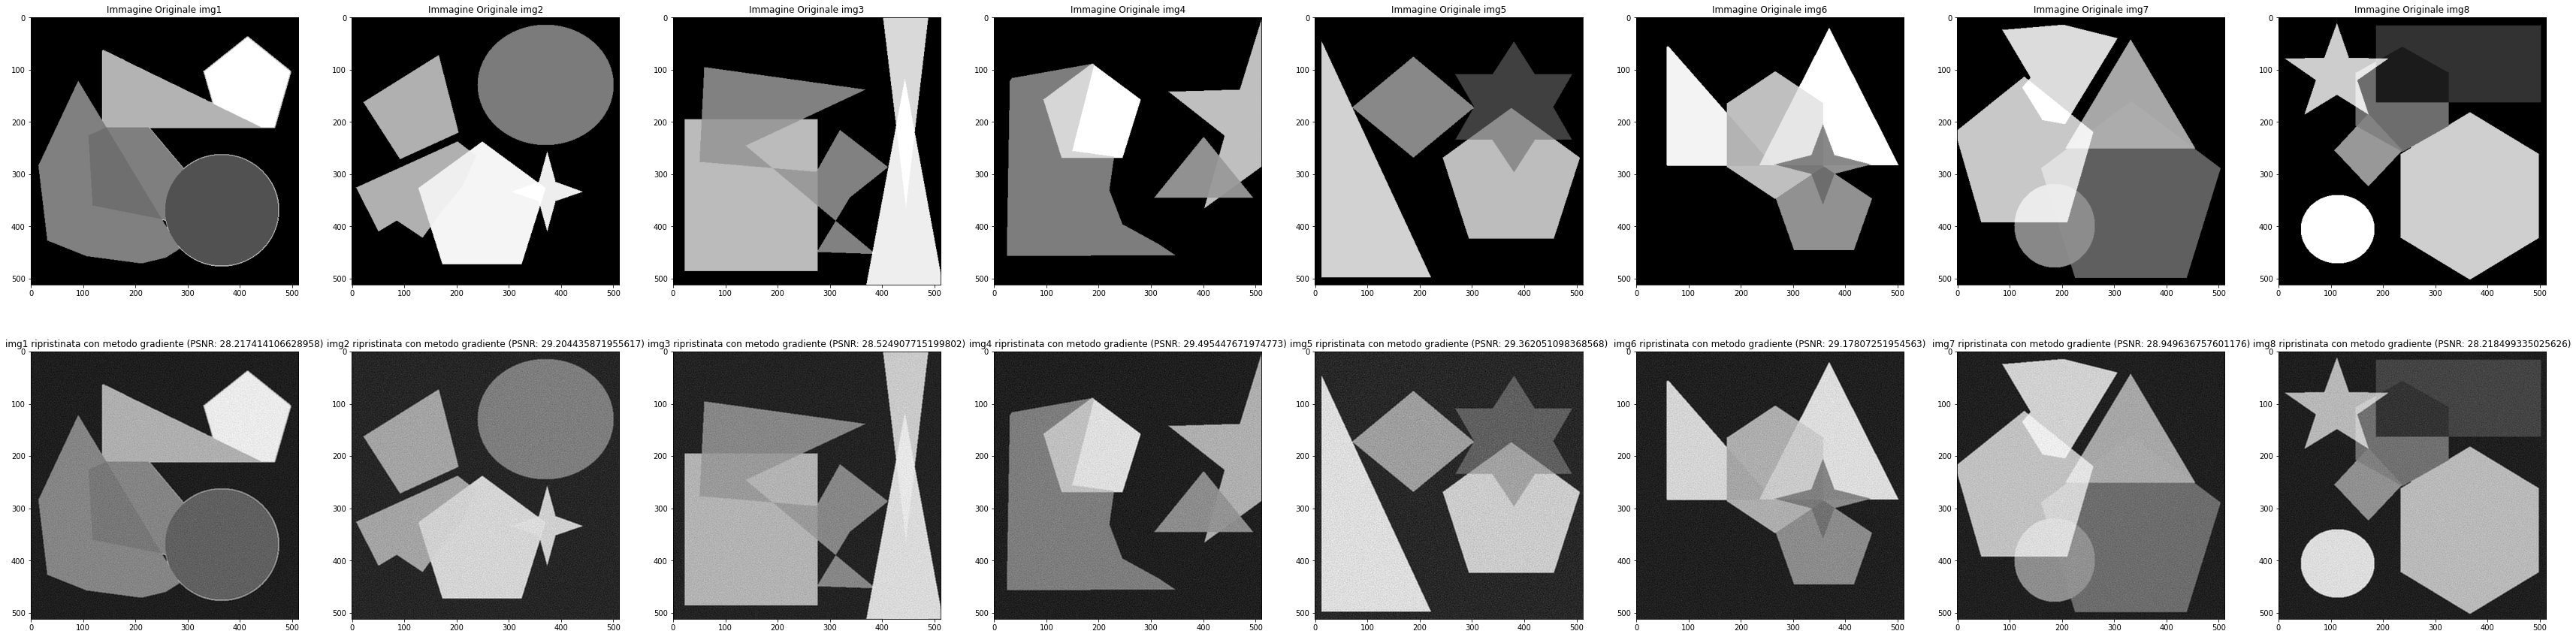
\includegraphics[width=0.7\textwidth]{imgRel/datasetgradiente.png}
    \caption{Immagini geometriche ripristinate}
    \label{fig:geomgradiente}
    \end{subfigure}

    \begin{subfigure}{0.5\textwidth}
        \centering
    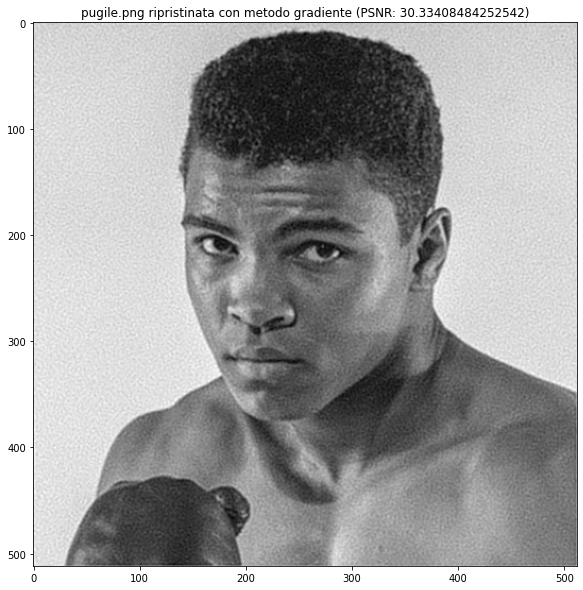
\includegraphics[width=0.6\linewidth]{imgRel/fotogrmg.png}
    \caption{Immagine fotografica ripristinata}
    \label{fig:pugilegradiente}
    \end{subfigure}%
    \begin{subfigure}{0.5\textwidth}\centering
        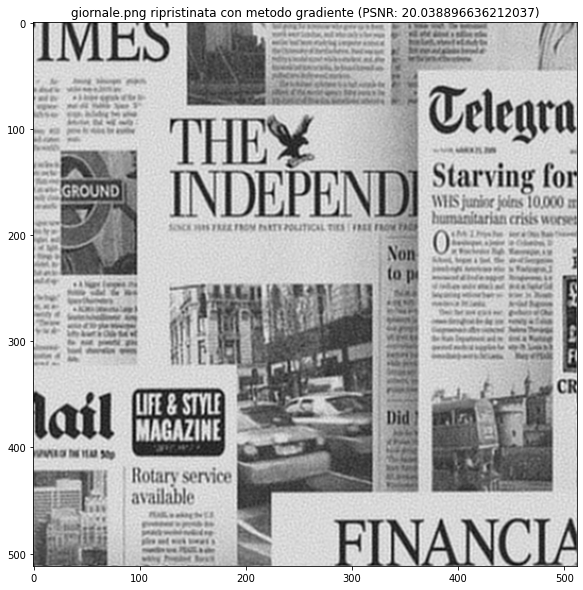
\includegraphics[width=0.6\linewidth]{imgRel/giornalemg.png}
        \caption{Immagine con testo ripristinata}
    \end{subfigure}
\caption{Immagini analizzate ripristinate con il Metodo del Gradiente}
    \centering
    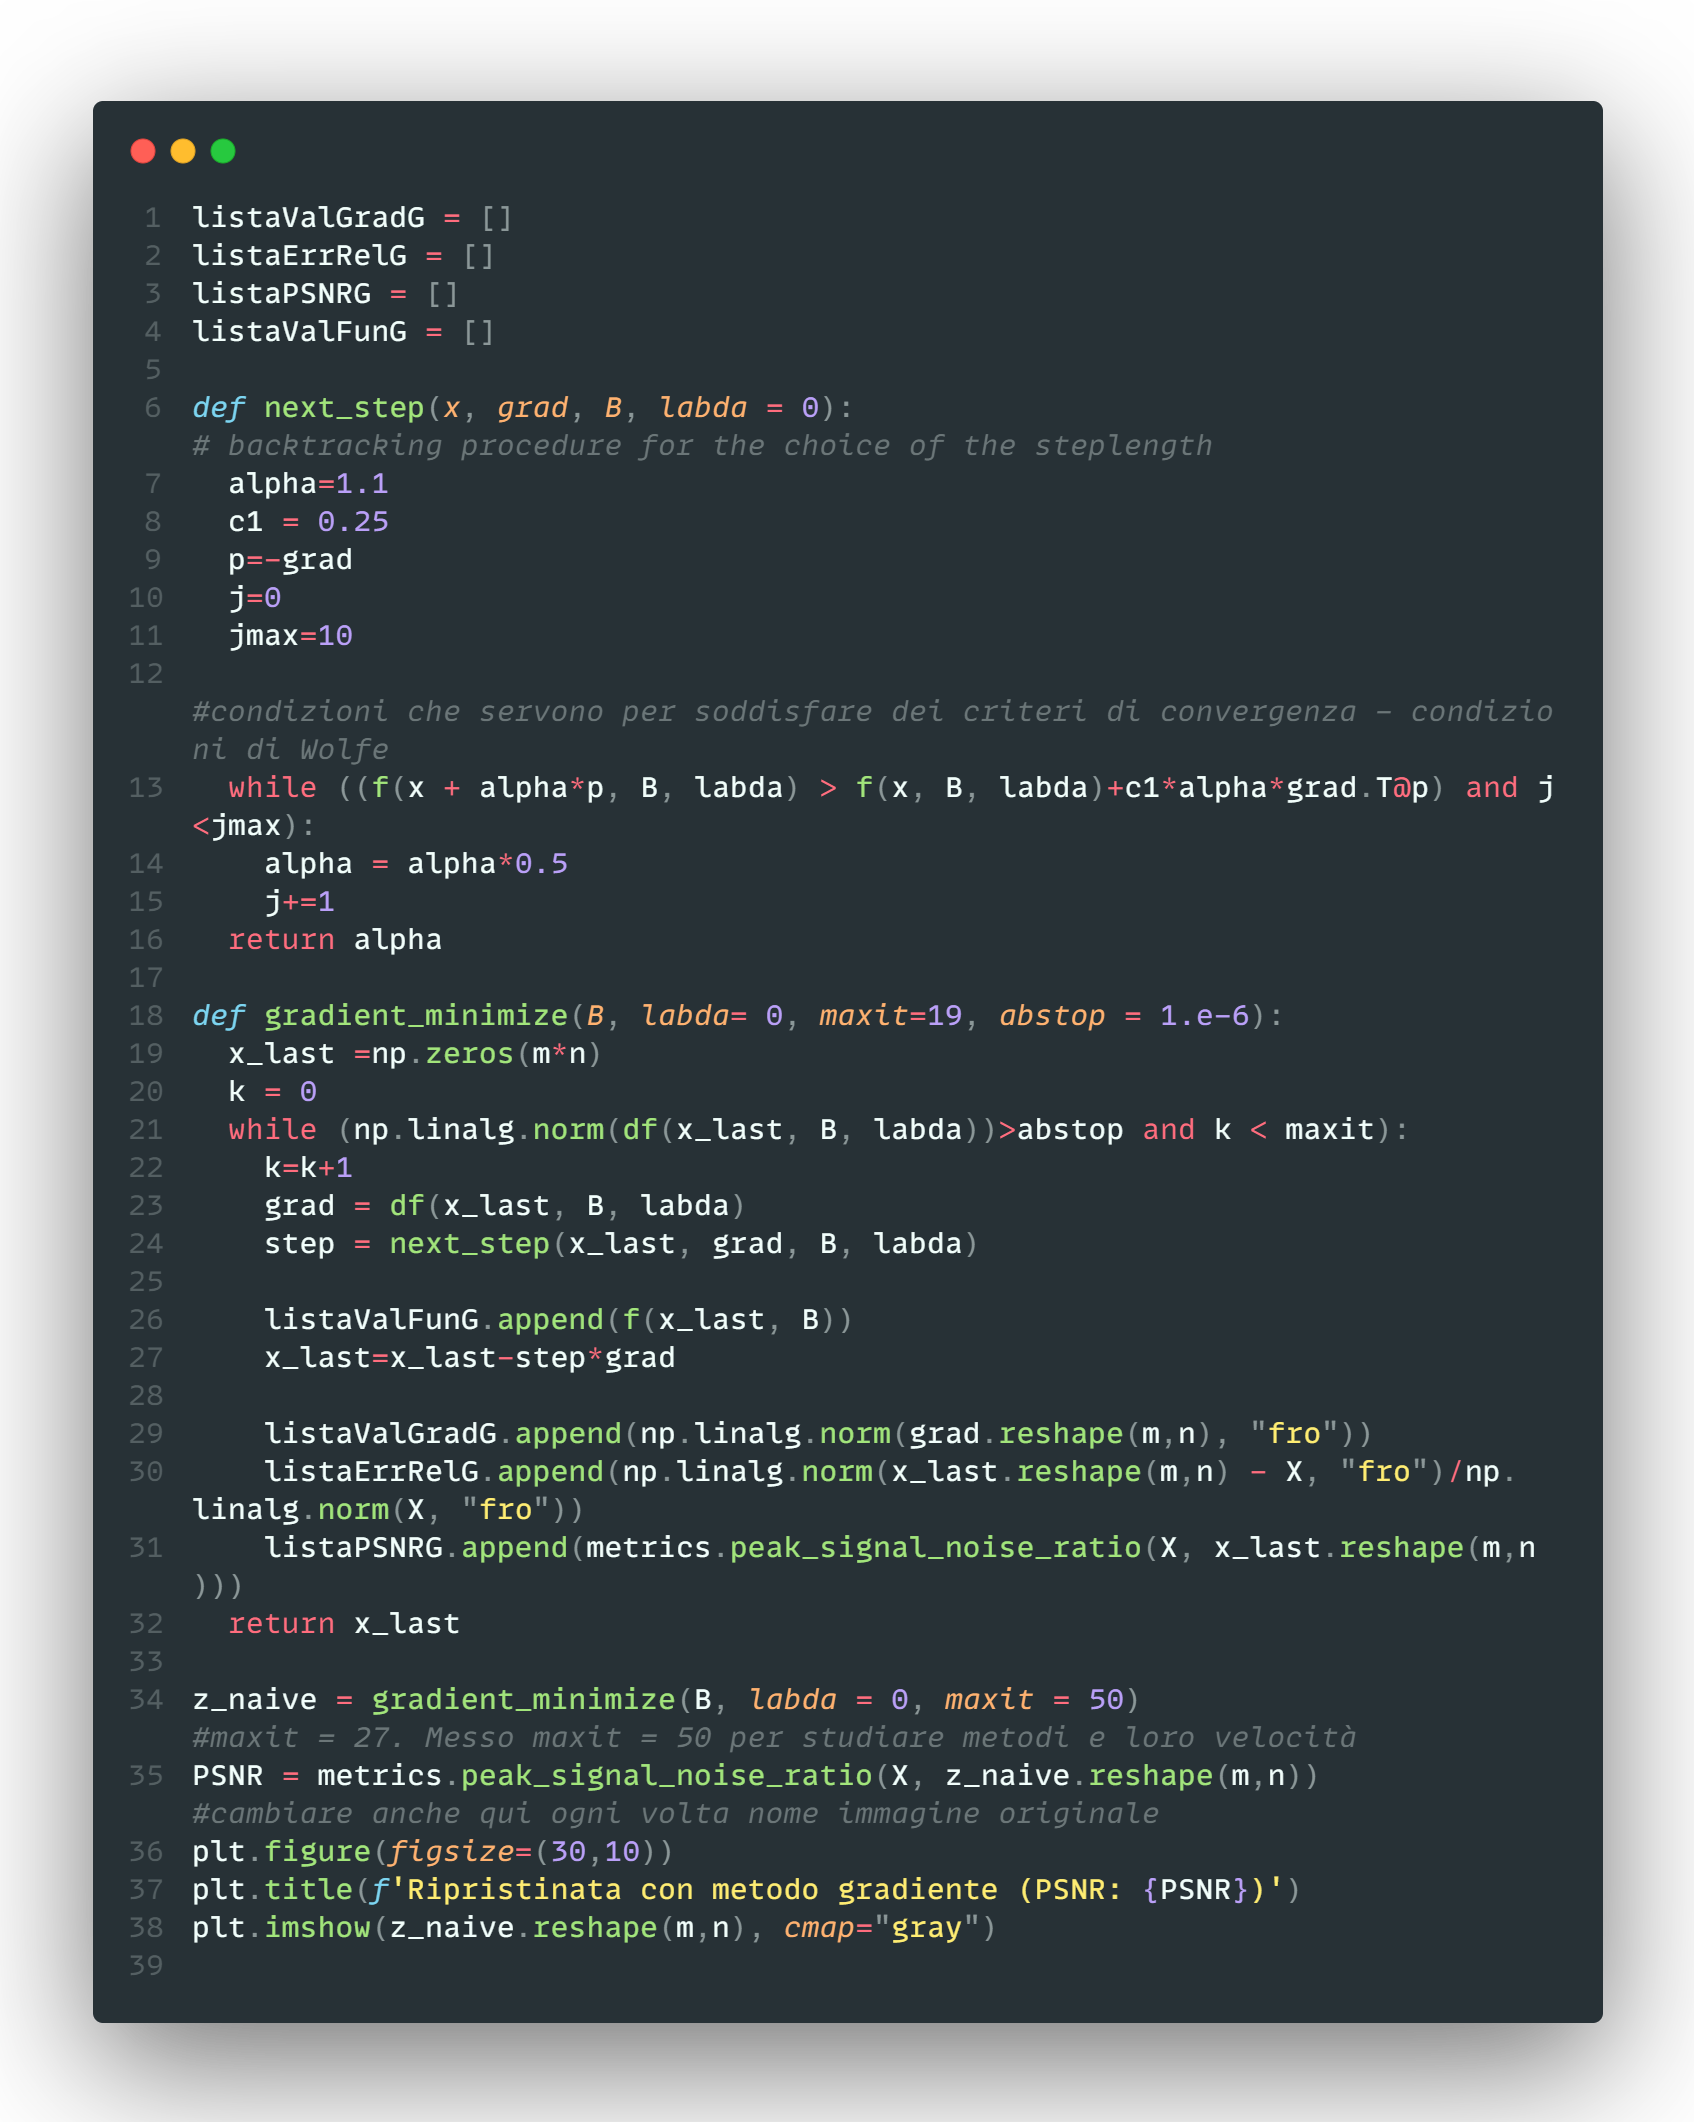
\includegraphics[width=0.7\textwidth]{imgCode/metGrad.png}
    \caption{Codice Metodo del gradiente applicato ad una singola immagine}
\end{figure}

